\chapter{Introduction}
\label{chap:introduction}

	\section{Overall description}
		The goal of this project is catching a ping pong ball released above a platform, on which four piezoelectric elements are placed in a rectangular pattern as shown in Figure \ref{fig:sideview}. Once the ball has hit the platform once, each of the piezo elements will generate a signal and permit triangulation of the impact point. When the impact point has been found, a net will catch the ball when it returns toward the platform after the first bounce.

		\begin{figure}[htb]
			\centering
			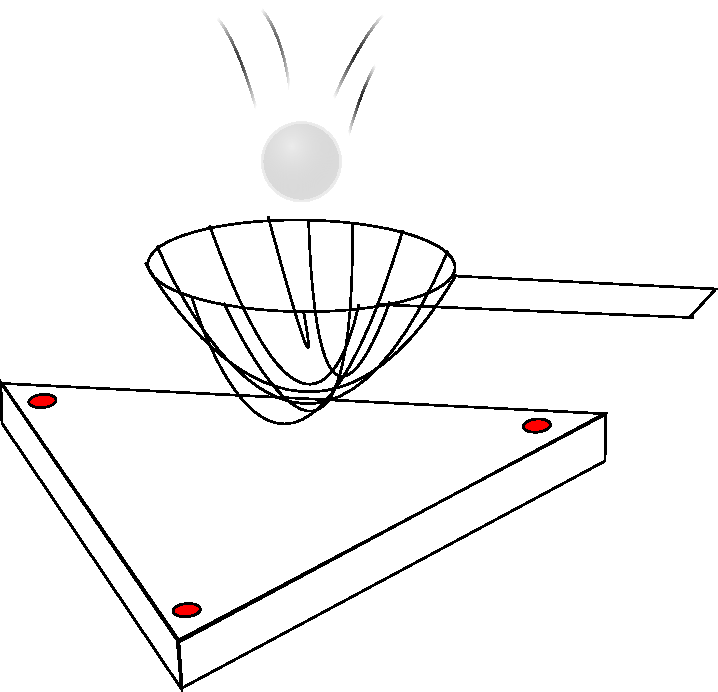
\includegraphics[width=0.8\textwidth]{figures/sideview}
			\caption{Side view of the platform surface area and the net. The red markings are piezoelectric sensors. TODO:change to picture of setup}
			\label{fig:sideview}
		\end{figure}

		Overall the different tasks of the project are thus:
		\begin{itemize}
			\item Calculating the xy-coordinate of the impact point
			\item Moving an arm -- holding a net -- to catch the ball after it has bounced once
		\end{itemize}

	\section{Report structure}
	\label{sec:reportStructure}
		\textcolor{red}{The report is structured as follows. To start the theoritical...}